% First generated, together with Chapter 8, as ch07_noisy_gates.tex by tools/conversion/make_ch07.py and since edited
% by hand (do not rerun it); see chapters/ch01_ch08_NOTES.md.
\chapter{Genuine and spurious fragility of quantum channel divergences near noisy gates}\label{gate:chapter}
\chaptermark{Fragility near noisy gates}
\begingroup
\chapmacro[1]{\dn}{\|#1\|_\diamond}
\chapmacro{\Fg}{\hat F}
\chapmacro{\FU}{F_{\mathrm U}}
\chapmacro{\DBS}{D_{\mathrm{BS}}}
\chapmacro{\lmin}{\lambda_{\min}}
\chapmacro{\lmax}{\lambda_{\max}}
\chapmacro{\Id}{\mathbf 1}
\chapmacro{\Dp}{\mathcal D_p}
\chapmacro{\cN}{\mathcal N}
\chapmacro{\cA}{\mathcal A}
\chapmacro{\IR}{F_{\mathrm{RLD}}}
\chapmacro{\IB}{F_{\mathrm{BKM}}}
\chapmacro{\IS}{F_{\mathrm{SLD}}}
\chapmacro{\Iinf}{F_{\infty}}
\chapmacro{\ltil}{\tilde\lambda}
\chapmathop{\vect}{vec}

\begin{chaptersummary}
Converse bounds on discriminating and estimating noisy quantum gates are evaluated on a characterized model of the gate. We ask whether their sensitivity to characterization error belongs to the task or only to the bound. The answer is governed by the noise floor $\ltil$, the smallest eigenvalue of the normalized Choi matrix. At first order, a diamond-norm error $\epsilon$ moves the geometric-fidelity and Belavkin--Staszewski converses for adaptive strategies by at most order $\epsilon/\ltil$, but at the worst case the adaptive exponents move equally, so this sensitivity is genuine. At second order, a coherent miscalibration $\delta$ of a gate with error probability $p$ moves these converses by order $\delta^2/p$, the Umegaki relative entropy by $\delta^2\ln(1/p)$, and the Uhlmann fidelity only by $\delta^2$, which is not amplified by the floor. Choi supports separate genuine jumps of the exponent from spurious ones, where converses are infinite while the exponent vanishes, as for the Chernoff exponent of amplitude damping. At a depolarized qubit gate the converses exceed the adaptive Stein and Chernoff exponents by at most a factor $3/2$ as $\delta\to0$, but by factors growing as $1/(\sqrt p\ln(1/p))$ near $\delta\approx2\sqrt p$. For $n$ qubits the fragile window of the converses scales as $p^{w/2}$ for an error of weight $w$; under biased noise it is set by the rate of the error itself. Certification through diamond-norm regions costs order $1/(\eta\ltil)^2$ uses for incoherent learners, variance-adaptive regions order $1/(\eta^2\ltil)$ for Pauli channels.
This opening chapter states the problem in physical terms and announces the results; the general theory behind them is developed in Chapters~\ref{cont:chapter}--\ref{chn:chapter}, and the proofs specific to noisy gates are in Chapter~\ref{gate:proofschapter}.
\end{chaptersummary}

\section{Introduction}\label{gate:sec:intro}

Before a quantum gate is used in a computation or a sensing protocol it is characterized. Randomized benchmarking, gate set tomography and process tomography produce a model of the gate together with error bars~\cite{Eisert2020,KlieschRoth2021,BlumeKohout2017}, and many statements about what the gate can do are then computed from that model. Among the most useful are converse bounds. They limit how well two gates can be told apart, or a parameter of a gate estimated, by any strategy, including adaptive ones that interleave the unknown gate with quantum memory and error correction~\cite{Hayashi2009,HHLW2010,Pirandola2019,KatariyaWilde2021,FangFawzi2021,ZhouJiang2021}. 
A claim that an error-corrected sensor operates at the precision limit set by its gates, or that an experiment demonstrates an advantage in discriminating two gates, is checked against such a bound. These bounds are single-letter: they are evaluated on one use of the channel, often as a semidefinite program, and they hold for any number of uses. A converse is therefore only as reliable as the model it is evaluated on, and its response to characterization error is a practical question.

For the converses that hold against adaptive strategies the response is poor. The geometric channel fidelity and the Belavkin--Staszewski relative entropy~\cite{BelavkinStaszewski1982,Matsumoto2018newf,FangFawzi2021,KatariyaWilde2021} are discontinuous at ideal unitary gates: the geometric fidelity of a gate with itself is one, but it vanishes against every miscalibrated copy, however close (Corollary~\ref{cont:cor:channels dichotomy} in Chapter~\ref{cont:chapter}). A real gate has an incoherent noise floor, which restores continuity, but the modulus of continuity then depends on the floor. For a depolarized single-qubit gate with error probability $p$, the $\delta^2$ coefficient of these divergences under a small coherent over-rotation $\delta$ grows as $1/p$, that of the Umegaki relative entropy as $\ln(1/p)$, and that of the Uhlmann fidelity stays of order one (Table~\ref{gate:tab:hier}). This is a different effect from the known gap between average infidelity and diamond distance~\cite{KuengLongDohertyFlammia2016}, which concerns the size of an error rather than the response of a bound to it. The floor is also the quantity that tomography resolves worst: for a two-qubit gate with $p=10^{-3}$ under local noise the normalized floor is about $6\times10^{-8}$, and a two-qubit $ZZ$ over-rotation of only $5\times10^{-4}$\,rad already reduces the geometric fidelity to $0.9$.

Is this sensitivity a defect of the bounds or a property of the tasks they bound? The question is not trivial, because the operational quantities are fragile too. Distinct unitaries can be discriminated perfectly with finitely many adaptive uses~\cite{DuanFengYing2007}, so adaptive error exponents jump at ideal gates. For a rotation under depolarizing noise, the Hamiltonian lies in the span of the products of Kraus operators, so error correction cannot restore Heisenberg scaling~\cite{DemkowiczDobrzanski2012,DemkowiczDobrzanski2017,ZZPJ2018,ZhouJiang2021}; it does, however, raise the asymptotic quantum Fisher information per use to order $1/p$~\cite{ZhouJiang2021,Dur2014,Kessler2014}. A converse valid for adaptive strategies must reproduce these features, but it need not be more sensitive than the task itself.

In this first chapter we separate the two effects. Part of the mathematical groundwork is developed later in the book, in Chapters~\ref{cont:chapter}, \ref{shA:chapter} and~\ref{chn:chapter}, whose results we use by forward reference, and the remaining proofs are collected in Chapter~\ref{gate:proofschapter}.
``Sensitivity'' has two meanings here, which we keep apart: the first-order change of a converse per unit of diamond-norm error in the model, and the second-order curvature of a converse in a coherent miscalibration $\delta$. Our main findings are the following.
\begin{enumerate}
\item The supports of the Choi matrices decide whether a jump is genuine (the exponent itself jumps), spurious (only the converse jumps) or absent. Amplitude damping, the standard model of energy relaxation, is genuine for the Stein exponent and spurious for the Chernoff exponent; a program-simulation converse stays finite there.
\item At first order, the geometric fidelity, the geometric Chernoff divergence and the Belavkin--Staszewski divergence obey a Choi-floor law: a diamond-norm error $\epsilon$ moves them by at most $\ln[1/(1-r)]$ with $r=\epsilon/(2\ltil)$, where $\ltil$ is the floor of the normalized Choi state. The resulting slope $1/(2\ltil)$ is sharp, and at the worst case the adaptive Stein and Chernoff exponents equal the converses and move at the same rate, so in this first-order sense the sensitivity belongs to the task.
\item At second order, the coefficients form the hierarchy of monotone metrics, and for $n$ qubits the fragile window is $\delta\sim p^{w/2}$ for a miscalibration of weight $w$. At a depolarized qubit gate the $1/p$ curvature of the Stein and Chernoff converses is genuine for $\delta\lesssim p\ln(1/p)$, where the ratio of converse to exponent is at most $3/2$ as $\delta\to0$, and spurious beyond, where the converse overshoots by a factor that grows as $p\to0$. Under biased single-qubit noise the local ratio stays below two; for correlated two-qubit errors it is open whether the exponent shares the window of the converse.
\item Certifying a geometric converse through a diamond-norm confidence region costs of order $1/(\eta\ltil)^2$ channel uses for accuracy $\eta$ with incoherent learners, whereas variance-adaptive confidence regions need only $O(1/(\eta^2\ltil))$ uses for Pauli channels.
\end{enumerate}
Figure~\ref{gate:fig:schematic} summarizes the classification and the scales on which it reappears at a noisy gate.

\begin{figure}[!tbp]
\centering
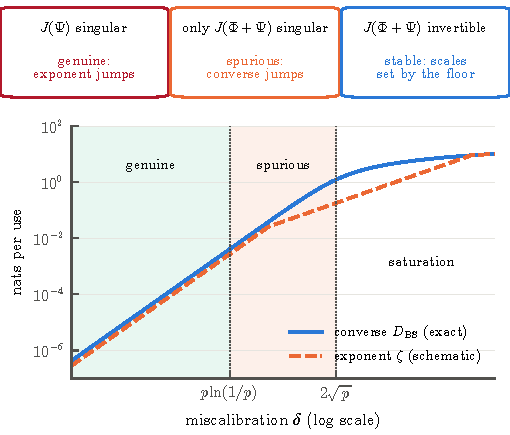
\includegraphics[width=0.8\linewidth]{fig0_schematic}
\caption{Schematic of the three regimes. Top: the supports of the Choi matrices decide whether a discontinuity is genuine (the operational exponent jumps), spurious (only single-letter converses jump) or absent. Bottom: at a stable pair, a depolarized qubit gate with $p=10^{-4}$ and a coherent miscalibration $\delta$, the distinction reappears on scales set by $p$. The solid line is the exact Belavkin--Staszewski converse; the dashed line is a schematic exponent that grows as $\delta^2/(3p)$ and then as $\delta\ln(1/p)$, illustrating the growth laws of Sec.~\ref{gate:sec:physical} (the certified bracket is in Fig.~\ref{gate:fig:crossover}). The converse follows the exponent for $\delta\lesssim p\ln(1/p)$, overshoots it up to $\delta\approx2\sqrt p$, and saturates beyond.}
\label{gate:fig:schematic}
\end{figure}

\section{Setting}\label{gate:sec:setting}

Let $\Phi,\Psi$ be quantum channels from an input space of dimension $d_X$ to an output space of dimension $d_Y$, with Choi matrices $J(\Phi)=\sum_{ij}\Phi(|i\rangle\langle j|)\otimes|i\rangle\langle j|$, so that $\Tr J(\Phi)=d_X$. The quantity that controls everything below is the \emph{Choi floor} $\lambda(\Psi)=\lmin(J(\Psi))$; the floor of the normalized Choi state is $\ltil=\lambda/d_X$. Distances between channels are measured in the unnormalized diamond norm $\dn{\cdot}$, so that $\dn{\Phi-\Psi}\le2$.

{\emergencystretch=6em The geometric fidelity is $\Fg(\Phi,\Psi)=\lmin\Tr_Y[J(\Phi)\#J(\Psi)]$, where $A\#B=A^{1/2}(A^{-1/2}BA^{-1/2})^{1/2}A^{1/2}$ is the Kubo--Ando geometric mean~\cite{KuboAndo1980} and $\Tr_Y$ the partial trace over the output~\cite{KatariyaWilde2021} (Proposition~\ref{cont:lambda min formula}). For singular arguments the mean is defined by continuity from above, $A\#B=\lim_{\varepsilon\downarrow0}(A+\varepsilon\Id)\#(B+\varepsilon\Id)$. The geometric Chernoff divergence $\hat C$ replaces $\#$ by the weighted means $\#_s$ and minimizes over $s\in[0,1]$, and the Belavkin--Staszewski (BS) divergence is $\DBS(\Phi\|\Psi)=\lmax\Tr_Y[J_\Phi^{1/2}\ln(J_\Phi^{1/2}J_\Psi^{-1}J_\Phi^{1/2})J_\Phi^{1/2}]$ with $J_\Phi=J(\Phi)$~\cite{BelavkinStaszewski1982,FangFawzi2021}.\par} The operational quantities are the adaptive Stein exponent $\zeta(\Phi\|\Psi)$, the decay rate of the type-II error at vanishing type-I error, and the adaptive Chernoff exponent $\xi(\Phi,\Psi)$ of the symmetric error. Both allow arbitrary adaptive strategies with quantum memory, which can outperform parallel ones~\cite{HHLW2010,SalekHayashiWinter2022}; $\zeta$ equals the regularized, or amortized, channel relative entropy~\cite{WangWilde2019,WBHK2020,FFRS2020}. The converses we study are
\begin{gather}
\zeta(\Phi\|\Psi)\le\DBS(\Phi\|\Psi),\label{gate:eq:converses}\\
\xi(\Phi,\Psi)\le\hat C(\Phi,\Psi)\le-2\ln\Fg(\Phi,\Psi),\label{gate:eq:converses2}
\end{gather}
from the chain rule of Fang and Fawzi~\cite{FangFawzi2021} and from Ref.~\cite{KatariyaWilde2021} and Theorem~\ref{chn:thm:main} and Corollary~\ref{chn:cor:compare} in Chapter~\ref{chn:chapter}. For comparison we use the Umegaki channel divergence $D(\Phi\|\Psi)$ and the Uhlmann channel root fidelity $\FU(\Phi,\Psi)$, optimized over inputs with a reference system. Neither gives an adaptive converse. The Umegaki divergence satisfies $D(\Phi\|\Psi)\le\zeta(\Phi\|\Psi)$~\cite{WangWilde2019,FFRS2020}, so it is a lower bound on the exponent, and $\FU$ stays close to one for close unitaries, which are perfectly distinguishable.

Our gate model is an $n$-qubit unitary $U$ with a coherent miscalibration $R_P(\delta)=e^{-i\delta P/2}$ about a Pauli string $P$ of weight $w$, followed by local depolarizing noise,
\begin{equation}\label{gate:eq:gate}
\cN_{p,\delta}=\Dp^{\otimes n}\circ\mathrm{Ad}_{R_P(\delta)}\circ\mathrm{Ad}_U,
\end{equation}
where $\Dp(\rho)=(1-p)\rho+p\Tr(\rho)\Id/2$, $\mathrm{Ad}_V(\rho)=V\rho V^\dagger$ and $\cN_p=\cN_{p,0}$. Its Choi floor is $\lambda=(p/2)^n$, i.e., $\ltil=(p/4)^n$, independently of $U$.

\section{Three regimes}\label{gate:sec:regimes}

Whether a divergence-based statement is continuous at a pair $(\Phi,\Psi)$ is decided by the supports of Choi matrices, and the operational exponents and their converses are decided by different ones. At the level of states, the analogous phenomenon is the discontinuity of the quantum Fisher information and of the Bures metric where the rank of the state changes~\cite{Safranek2017,Seveso2020}.

\emph{Genuine fragility.} The adaptive Stein exponent is continuous at $(\Phi,\Psi)$ if and only if $J(\Psi)$ is invertible or $\zeta(\Phi\|\Psi)=\infty$ (Corollary~\ref{shA:cor:stein}(c) in Chapter~\ref{shA:chapter}). At an ideal gate $U$, $\zeta(U\|U)=0$ but $\zeta(U'\|U)=\infty$ for every $U'\neq U$, and the same holds for $\xi$~\cite{DuanFengYing2007}. Every valid converse must therefore jump at ideal gates. The same applies to zero-temperature amplitude damping $\cA_\gamma$, whose Choi matrix has rank two: for $\gamma\neq\gamma'$ the outputs $\rho_\gamma$ and $\rho_{\gamma'}$ of $\cA_\gamma$ and $\cA_{\gamma'}$ on a maximally entangled input satisfy $\mathrm{supp}\,\rho_\gamma\not\subseteq\mathrm{supp}\,\rho_{\gamma'}$, so $\zeta(\cA_\gamma\|\cA_{\gamma'})=\infty$. A model with pure $T_1$ decay thus predicts, for any two damping rates, a type-II error that decays faster than any exponential. In this case the discontinuity lies in the model itself.

\emph{Spurious fragility.} As functions on pairs of completely positive maps, the geometric quantities are continuous at $(\Phi,\Psi)$ if and only if $J(\Phi+\Psi)$ is invertible or $\Fg(\Phi,\Psi)=0$ (Theorem~\ref{cont:thm:dichotomy} in Chapter~\ref{cont:chapter}). Within channels, this dichotomy is proved at the diagonal pairs $(\Phi,\Phi)$, which are continuity points if and only if $J(\Phi)$ is invertible (Corollary~\ref{cont:cor:diagonal channels}); for other channel pairs with $J(\Phi+\Psi)$ singular and $\Fg>0$ it is open. The divergence $\hat C$ is continuous wherever $J(\Phi+\Psi)$ is invertible (Theorem~\ref{chn:thm:semicont}(c) in Chapter~\ref{chn:chapter} and Proposition~\ref{gate:smp:prop:cont} in Chapter~\ref{gate:proofschapter}). When $J(\Phi+\Psi)$ is singular but the true exponent is finite, a converse can jump while the exponent does not. Amplitude damping provides the physical example~\cite{RexitiMancini2021}. For $\gamma\neq\gamma'$ one has $\Fg(\cA_\gamma,\cA_{\gamma'})=0$, so $\hat C$, $-2\ln\Fg$ and the barycentric converse $C_{\rm bar}$ of Ref.~\cite{JMMW2024} are all infinite (Proposition~\ref{chn:prop:adlevels}), whereas the true Chernoff exponent tends to zero as $\gamma'\to\gamma$. The infinite value is a property of the Choi-level geometric mean and is witnessed by the input $|0\rangle$, on which both channels act identically, so it carries no physical information. With $\Delta=\gamma-\gamma'$ we find (see Chapter~\ref{gate:proofschapter}, Section~\ref{gate:sec:ad})
\begin{gather}
\xi_{\rm prod}\le\xi(\cA_\gamma,\cA_{\gamma'})\le-2\ln\mu_*,\label{gate:eq:ad}\\
\mu_*=\frac{\sqrt{\gamma\gamma'}}{1-\sqrt{(1-\gamma)(1-\gamma')}},\nonumber
\end{gather}
where $\xi_{\rm prod}$ is the classical Chernoff information of the outputs $\mathrm{diag}(\gamma,1-\gamma)$ and $\mathrm{diag}(\gamma',1-\gamma')$ on the product input $|1\rangle$. To leading order in $\Delta$, $\xi_{\rm prod}\simeq\Delta^2/[8\gamma(1-\gamma)]$ and $-2\ln\mu_*\simeq\Delta^2/[4\gamma^2(1-\gamma)]$. The upper bound comes from a converse that applies to any pair of channels: $\mu_*$ is the largest overlap of two pure program states from which a common channel simulates both channels, as in the programmable simulations of Refs.~\cite{PirandolaLupo2017,Pirandola2019}; it is a semidefinite program for any pair, and the error of any adaptive strategy is at least $\frac14\mu_*^{2n}$ after $n$ uses. For $n\le4$ uses, exact semidefinite programs give the minimal root fidelity of the two final states as $f^n$, where $f$ is the Bhattacharyya coefficient of the two damping probabilities. This suggests the sharper bound $\xi\le-2\ln f$ [Fig.~\ref{gate:fig:regimes}(a)].

Replacement channels, which output a fixed state, give a second example. There are pairs $\Phi_t,\Psi_t$ at diamond distance $O(\sqrt t)$ from a pair of identical channels for which $\hat C$, $-2\ln\Fg$ and $C_{\rm bar}$ are infinite for every $t>0$, while $\xi=2\ln[(1+t)/(1-t)]\approx4t$ exactly [Theorem~\ref{gate:smp:thm:fragile} in Chapter~\ref{gate:proofschapter} and the example after it; Fig.~\ref{gate:fig:regimes}(b)]; the parameter $t$ controls the overlap of the two output states. Here the program-simulation converse is tight, $-2\ln\mu_*=\xi$, so the jump is an artifact of $\hat C$, $-2\ln\Fg$ and $C_{\rm bar}$ alone.

\begin{figure}[!tbp]
\centering
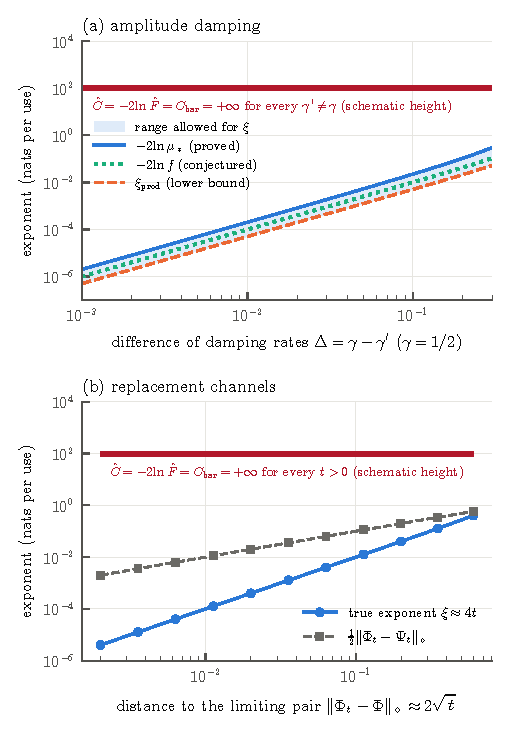
\includegraphics[width=0.8\linewidth]{fig1_regimes}
\caption{Spurious fragility of single-letter Chernoff converses. (a) Amplitude damping $\cA_\gamma$ against $\cA_{\gamma'}$ at $\gamma=1/2$, as a function of $\Delta=\gamma-\gamma'$. The converses $\hat C$, $-2\ln\Fg$ and $C_{\rm bar}$ are infinite for every $\Delta\neq0$ (thick line, drawn at a schematic height). The true adaptive Chernoff exponent $\xi$ lies in the shaded range between the product-input lower bound $\xi_{\rm prod}$ (dashed) and the program-simulation upper bound $-2\ln\mu_*$ of Eq.~\eqref{gate:eq:ad} (solid); the dotted line is the conjectured bound $-2\ln f$. (b) Replacement channels $\Phi_t,\Psi_t$ with outputs $\phi_t,\psi_t$, which converge to a common state as $t\to0$, against the diamond distance to the limiting pair. The converses are again infinite, whereas the true exponent, the quantum Chernoff bound of $\phi_t$ and $\psi_t$, is $\xi=2\ln[(1+t)/(1-t)]\approx4t$ (circles), which here equals the program-simulation bound $-2\ln\mu_*$; squares show $\frac12\dn{\Phi_t-\Psi_t}$ for comparison. In both cases the converses are infinite while the exponent tends to zero.}
\label{gate:fig:regimes}
\end{figure}

\emph{Stable pairs.} When $J(\Phi+\Psi)$ is invertible, all the quantities above are continuous (Theorem~\ref{cont:thm:dichotomy}(a), Theorem~\ref{chn:thm:semicont}(c), Proposition~\ref{gate:smp:prop:cont} and Remark~\ref{gate:smp:rem:zeta} in Chapter~\ref{gate:proofschapter}; for $\DBS$, Remark~\ref{gate:smp:rem:dbs}, which derives it from Theorem~\ref{cont:thm:four maps}(e) and Corollary~\ref{cont:cor:dmax growth}). Every channel of full Kraus rank, and so every gate model with a nonzero depolarizing or thermal floor, falls in this class. Divergences built directly from hypothesis tests, such as the hockey-stick divergences and their integrals~\cite{HircheTomamichel2024,HMT2026}, are even uniformly continuous with dimension-free moduli (Theorem~\ref{shA:thm:bounded} and Corollary~\ref{shA:cor:nodichotomy} in Chapter~\ref{shA:chapter}), but they do not give adaptive converses. Near realistic gates the classification is therefore only qualitative, and the rest of this chapter makes it quantitative.

\section{First-order sensitivity: the Choi-floor law}\label{gate:sec:laws}

The basic step converts a diamond-norm error into a relative error of Choi matrices. For two channels, $\|J(\Phi)-J(\Phi')\|_\infty\le\frac{d_X}{2}\dn{\Phi-\Phi'}$, with equality attained in every dimension (Lemma~\ref{gate:lem:J} in Chapter~\ref{gate:proofschapter}). Hence a channel $\Psi'$ within diamond distance $\epsilon$ of $\Psi$ satisfies $(1-r)J(\Psi)\le J(\Psi')\le(1+r)J(\Psi)$ in the positive semidefinite order, with relative radius
\begin{equation}\label{gate:eq:r}
r=\frac{d_X\,\epsilon}{2\lambda(\Psi)}=\frac{\epsilon}{2\ltil(\Psi)} .
\end{equation}
Combined with the monotonicity and homogeneity of Kubo--Ando means, and with the operator monotonicity of the logarithm, this gives the following result.

\begin{theorem}[Choi-floor law]\label{gate:thm:floor}
Let $\Psi,\Psi'$ be channels with $\dn{\Psi'-\Psi}\le\epsilon$ and $r<1$ as in Eq.~\eqref{gate:eq:r}. For every completely positive map $\Phi$,
\begin{gather}
\sqrt{1-r}\;\Fg(\Phi,\Psi)\le\Fg(\Phi,\Psi')\le\sqrt{1+r}\;\Fg(\Phi,\Psi),\label{gate:eq:floor}\\
|\hat C(\Phi,\Psi')-\hat C(\Phi,\Psi)|\le\ln\frac1{1-r},\nonumber
\end{gather}
and for every channel $\Phi$, $-\ln(1+r)\le\DBS(\Phi\|\Psi')-\DBS(\Phi\|\Psi)\le\ln[1/(1-r)]$. If $d_X=d_Y$ and the $\lambda$-eigenspace of $J(\Psi)$ contains a maximally entangled vector, as for every Pauli channel composed with a unitary, the constants are sharp. For $\ln\Fg$,
\begin{equation}\label{gate:eq:sharp}
\sup_\Phi\ \limsup_{\epsilon\to0}\ \sup_{\dn{\Psi'-\Psi}\le\epsilon}\frac{|\ln\Fg(\Phi,\Psi')-\ln\Fg(\Phi,\Psi)|}{\epsilon}=\frac{1}{4\ltil},
\end{equation}
and at the same $\Phi$ the bounds for $\hat C$ and $\DBS$ are attained to first order.
\end{theorem}

The worst case is a unitary $\Phi=\mathrm{Ad}_W$ whose Choi vector lies in the floor eigenspace, perturbed towards any unitary $W'$ with $\Tr W^\dagger W'=0$. For local noise, $W$ differs from the gate by a correlated error of full weight. Only the floor of the perturbed argument enters; a two-sided version in which both channels move holds with $1\pm r$ in place of $\sqrt{1\pm r}$ (Theorem~\ref{cont:thm:choi floor} in Chapter~\ref{cont:chapter}; Proposition~\ref{gate:smp:prop:twosided} in Chapter~\ref{gate:proofschapter} allows separate floors). At this worst case $\hat C=\DBS=-2\ln\Fg=\ln(1/\ltil)$ (Proposition~\ref{gate:prop:worst} below), so the three bounds of Theorem~\ref{gate:thm:floor} are attained together, with slope $1/(2\ltil)$ for $\hat C$, $\DBS$ and $-2\ln\Fg$. At a depolarized qubit gate, $1/(4\ltil)=1/p$, so for the worst-case $\Phi$ a diamond-norm error $\epsilon$ can move $-2\ln\Fg$ by $2\epsilon/p$. In absolute terms the largest slope of $\Fg$ itself lies between $[2/(3\sqrt3\,p)][1+o(1)]\approx0.385/p$, attained by a unitary $\Phi$, and $1/p$. We conjecture that unitary $\Phi$ are the worst case; a numerical search over mixed $\Phi$ found nothing larger. The maximizing unitary sits at a pair where the converse already overshoots the Stein exponent, by a certified factor of at least $5$ at $p=10^{-3}$ (Table~\ref{gate:tab:m1L2}), so this absolute slope is a property of the converse.

The Stein exponent behaves differently in the channel under test. Errors of size $\epsilon'=\frac12\dn{\Phi-\Phi'}$ in $\Phi$ change $\zeta$ by at most $2\epsilon'\ln d_Y+(1+\epsilon')h(\epsilon'/(1+\epsilon'))+\epsilon'\ln\kappa(\Psi)$, where $h$ is the binary entropy and $\kappa(\Psi)$ the condition number of $J(\Psi)$ (Corollary~\ref{shA:cor:stein} in Chapter~\ref{shA:chapter}). Near a gate $\kappa\simeq(4/p)^n$, so this modulus grows only as $\ln(1/p)$. Errors in the reference channel $\Psi$ enter $\zeta$ through the Thompson metric between $J(\Psi)$ and $J(\Psi')$, which is at most $\ln[1/(1-r)]$~\cite{Thompson1963} (Theorem~\ref{shA:thm:thompson}, and Eq.~\eqref{gate:eq:Ssandwich} in Chapter~\ref{gate:proofschapter}). In fact, every quantity considered here, the exponents $\zeta$ and $\xi$ included, is 1-Lipschitz in the Thompson metric, so none of them moves by more than $\ln[1/(1-r)]$ under such an error (Proposition~\ref{gate:prop:m1thompson}). Section~\ref{gate:sec:physical} shows that the exponents attain this rate at the worst case of Theorem~\ref{gate:thm:floor}.

\begin{table}[!tbp]
\centering
\caption{Second-order response of channel divergences to a coherent over-rotation $\delta$ at a depolarized qubit gate, $\cN_{p,\delta}$ against $\cN_p$ with $P=Z$: coefficients of $\delta^2$. Each coefficient is a Fisher information per use of one monotone metric; the last row is the asymptotic Fisher information with adaptive control and error correction. All entries are exact. $D$ and $\FU$ use the maximally entangled input, which is optimal.}
\label{gate:tab:hier}
\begin{tabular}{lll}
\toprule
quantity & coefficient of $\delta^2$ & $p\to0$\\
\midrule
$1-\Fg$ & $\IR/8$ & $1/(8p)$\\
$\DBS(\cN_{p,\delta}\|\cN_p)$ & $\IR/2$ & $1/(2p)$\\
$D(\cN_{p,\delta}\|\cN_p)$ & $\IB/2$ & $\ln(4/p)/4$\\
$1-\FU(\cN_{p,\delta},\cN_p)$ & $\IS/8$ & $1/8$\\
\midrule
$\IR$ (RLD) & \multicolumn{2}{l}{$2(1-p)^2(2-p)/[p(4-3p)]$}\\
$\IB$ (BKM) & \multicolumn{2}{l}{$\frac12(1-p)\ln[(4-3p)/p]$}\\
$\IS$ (SLD) & \multicolumn{2}{l}{$2(1-p)^2/(2-p)$}\\
$\Iinf$ (adaptive) & \multicolumn{2}{l}{$2(1-p)^2/[p(3-2p)]$}\\
\bottomrule
\end{tabular}
\end{table}

\section{Second-order sensitivity: monotone metrics and the multi-qubit window}\label{gate:sec:second}

Theorem~\ref{gate:thm:floor} is a worst case over pairs. At a given pair, such as a gate and its miscalibrated copy, the response is governed by curvature. The hierarchy in Table~\ref{gate:tab:hier} has a simple interpretation. To second order, each divergence is a monotone Riemannian metric~\cite{Petz1996} evaluated on the Choi state: the right logarithmic derivative (RLD) metric for $\Fg$ and $\DBS$, the Bogoliubov--Kubo--Mori (BKM) metric for $D$, and the symmetric logarithmic derivative (SLD) metric for $\FU$~\cite{Petz1996,BraunsteinCaves1994,KatariyaWilde2021b}. A coherent error couples the top eigenvector of the Choi state, with eigenvalue $\mu\approx1$, to a floor eigenvector with eigenvalue $\ltil$. The metric defined by an operator monotone function $f$ weights such a coherence by $c_f(\mu,\ltil)=1/[\mu f(\ltil/\mu)]$, which is $(\mu+\ltil)/(2\mu\ltil)$ for RLD, $\ln(\mu/\ltil)/(\mu-\ltil)$ for BKM and $2/(\mu+\ltil)$ for SLD. The weight stays bounded as $\ltil\to0$ exactly when $f(0^+)>0$. Two caveats matter in practice. The Uhlmann fidelity is not amplified by the floor for coherent errors, but an incoherent change of a floor eigenvalue costs $1/\ltil$ in every metric; at the worst case of Theorem~\ref{gate:thm:floor} the Umegaki divergence and the Uhlmann fidelity equal the converses and have the same first-order sensitivity (Proposition~\ref{gate:prop:worst}). The hierarchy is therefore a statement about the second-order response to coherent errors only. And the closed forms extend to any Pauli channel, any Pauli-string miscalibration and any $n$ (Theorem~\ref{gate:thm:B} in Chapter~\ref{gate:proofschapter}).

For $n$ qubits the floor $\ltil=(p/4)^n$ is exponentially small, and which errors reach it depends on their weight. For $\cN_{p,\delta}$ of Eq.~\eqref{gate:eq:gate},
\begin{equation}\label{gate:eq:window}
\Bigl(1-\tfrac{3p}{4}\Bigr)^{n}g(x)\le1-\Fg(\cN_{p,\delta},\cN_p)\le g(x),
\end{equation}
where $g(x)=1-(1+x)^{-1/2}$, $x=(\kappa_w-1)^2\sin^2(\delta/2)/(4\kappa_w)$, and $\kappa_w=[(4-3p)/p]^w$ is the ratio of the two Choi eigenvalues coupled by the error; for $w=n$ it is the condition number of $J(\cN_p)$. The geometric infidelity therefore reaches a level $\eta$ at the window
\begin{equation}\label{gate:eq:delta}
\delta_\eta=4\sqrt{x_\eta}\,\Bigl(\frac p4\Bigr)^{w/2}\bigl[1+O(np)\bigr],
\end{equation}
with $x_\eta=(1-\eta)^{-2}-1$, and $\DBS$ obeys the same scaling. The window depends on the weight of the error, not on the number of qubits: a weight-one error on any number of qubits has $\delta_{0.1}\approx0.97\sqrt p$. A full-weight error has $\delta_\eta\propto p^{n/2}$. At $p=10^{-3}$ and $\eta=0.1$ this is $\delta_\eta\approx4.8\times10^{-4}$ for a two-qubit $ZZ$ error and $1.2\times10^{-7}$ for a four-qubit error of full weight. Under global depolarizing noise of the same strength the window is $\delta_\eta\simeq4\sqrt{x_\eta p}/d$, with $d=2^n$, which is $1.5\times10^{-2}$ for two qubits. By contrast $D\le w\ln[(4-3p)/p]\sin^2(\delta/2)$ and $1-\FU\le\sin^2(\delta/2)$, independently of $n$. The worst-case modulus of Theorem~\ref{gate:thm:floor} at this gate, taken over the other argument, is $\frac14(4/p)^n$. Figure~\ref{gate:fig:window} shows the collapse of exact evaluations for $n=1,2,3$.

\emph{Biased noise.} The closed forms cover any Pauli noise (Chapter~\ref{gate:proofschapter}, Section~\ref{gate:sec:biased}). For a miscalibration about $P$ the window is set by the coupled rate $q_P$, the probability of the Pauli error $P$ itself, as $\delta_\eta\simeq4\sqrt{x_\eta q_P/q_{\Id}}$, whereas the floor $\ltil=\min_Qq_Q$ sets the worst-case modulus of Theorem~\ref{gate:thm:floor}; the two are set by different rates. Under dephasing-dominated noise with bias $b=p_z/(p_x+p_y)$, as in bias-preserving architectures~\cite{Tuckett2018,Puri2020}, a $Z$ miscalibration keeps the wide window $1.94\sqrt{p_z}$ for every $b$, whereas the window of an $X$ miscalibration narrows to $1.94\sqrt{p_z/(2b)}$, set by the small transverse rate.

\begin{figure}[!tbp]
\centering
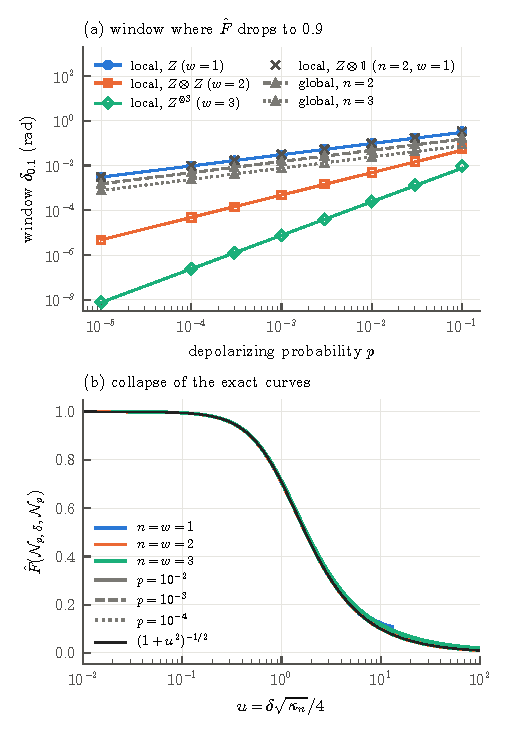
\includegraphics[width=0.8\linewidth]{fig2_window}
\caption{Fragility window of the geometric fidelity for $n=1,2,3$ qubits. (a) Miscalibration $\delta_{0.1}$ at which $\Fg(\cN_{p,\delta},\cN_p)$ drops to $0.9$, from exact 50-digit evaluations (symbols), for local depolarizing noise with a miscalibration of weight $w$ (colors) and for global depolarizing noise (grey). Lines are the asymptotic laws $1.94\,(p/4)^{w/2}$ and $1.94\sqrt p/d$; fitted slopes for $p\le10^{-3}$ are $0.500$, $1.000$ and $1.500$ for $w=1,2,3$. The weight-one error $Z\otimes\Id$ on two qubits (crosses) has the same window as $Z$ on one qubit. (b) The exact curves for $w=n$ and $p=10^{-2},10^{-3},10^{-4}$, plotted against $u=\delta\sqrt{\kappa_n}/4$, collapse onto $(1+u^2)^{-1/2}$; here $\kappa_n=[(4-3p)/p]^n$ is both the ratio of the two coupled Choi eigenvalues and the condition number of $J(\cN_p)$. The fragile window of an $n$-qubit gate is set by the weight of the error and is exponentially small in it.}
\label{gate:fig:window}
\end{figure}

\begin{figure}[!tbp]
\centering
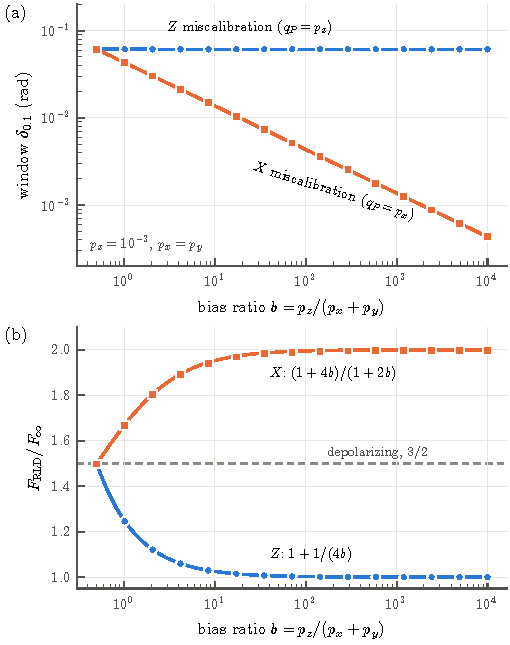
\includegraphics[width=0.8\linewidth]{biased_window_ratio}
\caption{Biased qubit noise with $p_z=10^{-3}$ and $p_x=p_y$, against the bias ratio $b=p_z/(p_x+p_y)$; $b=\frac12$ is depolarizing noise. (a) Window $\delta_{0.1}$ at which $\Fg(\cN_\delta,\cN_0)=0.9$, for $Z$ miscalibrations (circles) and $X$ miscalibrations (squares); markers are exact, lines the law $\delta_{0.1}=1.937\sqrt{q_P/q_\Id}$. (b) The ratio $\IR/\Iinf$, which bounds $\limsup_{\delta\to0}\DBS/\zeta$; lines are the leading-order laws $1+1/(4b)$ ($Z$) and $(1+4b)/(1+2b)$ ($X$), and the dashed line is the depolarizing value $3/2$. Errors aligned with the bias keep a wide window and a converse within $3/2$ of the exponent; misaligned errors have a narrow window and a gap that approaches two.}
\label{gate:fig:biased}
\end{figure}

\section{Genuine and spurious parts of the fragility}\label{gate:sec:physical}

We now compare the converses with the exponents they bound, first at first order and then at second order.

\emph{First order.} At the worst case of Theorem~\ref{gate:thm:floor} the converses are exact.

\begin{proposition}[Genuine first-order fragility]\label{gate:prop:worst}
Let $d_X=d_Y$, let $\Psi$ be a channel with $J(\Psi)>0$, and let $W$ be a unitary whose Choi vector is an eigenvector of $J(\Psi)$ with eigenvalue $d_X\tilde\mu$. Then
\begin{equation}\label{gate:eq:worst}
\zeta=\xi=\DBS=\hat C=-2\ln\Fg=D=-2\ln\FU=\ln(1/\tilde\mu),
\end{equation}
all evaluated at $(\mathrm{Ad}_W,\Psi)$. All seven quantities have the same derivative in every direction of $\Psi$, so for a floor eigenvector ($\tilde\mu=\ltil$) each of them changes at the rate $1/(2\ltil)$ per unit of diamond distance, the sharp rate of Theorem~\ref{gate:thm:floor}.
\end{proposition}

The optimal test is a Bell measurement in the frame of $W$, which detects every error other than $W$; for a Pauli channel $\tilde\mu=q_W$, and Eq.~\eqref{gate:eq:worst} holds exactly at every Pauli channel in the same frame. The sharp constant of Theorem~\ref{gate:thm:floor} is therefore a property of the task: the floor sets the error budget for any statement about discriminating a gate from the model $\Psi$. More generally, wherever a converse is tight and differentiable, the exponent is at least as sensitive at first order as the converse, so a first-order spurious gap can occur only where the converse already overestimates the exponent (Lemma~\ref{gate:lem:m1tight} in Chapter~\ref{gate:proofschapter}). For Pauli-diagonal pairs the single-letter converses are exact (Proposition~\ref{gate:prop:m1pauli}), whereas at the slope maximizer of Sec.~\ref{gate:sec:laws} they are not.

\emph{Second order.} We compare the BS converse with the exponent it bounds, $\zeta(\cN_{p,\delta}\|\cN_p)$, for the qubit gate ($n=1$, $P=Z$). At small $\delta$ the comparison can be made exactly. Any fixed $k$-use strategy gives $\zeta\ge\frac1kD(\rho_k^\delta\|\rho_k^0)$, where $\rho_k^\delta$ are its output states~\cite{WangWilde2019,FFRS2020}. Because $J(\cN_{p,\delta})\ge(p/2)\Id$, these outputs have $\delta$-independent support, and the relative entropy is, to second order, a BKM metric, which dominates the SLD metric~\cite{Petz1996}. Taking the error-corrected strategies of Zhou and Jiang~\cite{ZhouJiang2021} gives $\liminf_{\delta\to0}\zeta/\delta^2\ge\Iinf/2$, where $\Iinf$ is the asymptotic Fisher information per use. For this gate the Hamiltonian lies in $\mathrm{span}\{K_i^\dagger K_j\}$, where $K_i$ are the Kraus operators, so the scaling is linear, and $\Iinf=2(1-p)^2/[p(3-2p)]$; this is the closed form of Ref.~\cite{ZhouJiang2021}, and a primal--dual pair of the corresponding semidefinite program, evaluated in 50-digit arithmetic, agrees with it to a relative gap below $2\times10^{-47}$ (Chapter~\ref{gate:proofschapter}, Section~\ref{gate:sec:local}). Since $\DBS=\IR\delta^2/2+O(\delta^4/p^2)$, our result for the local regime is
\begin{equation}\label{gate:eq:ratio}
\begin{split}
1\le\liminf_{\delta\to0}\frac{\DBS}{\zeta}&\le\limsup_{\delta\to0}\frac{\DBS}{\zeta}\\
&\le\frac{\IR}{\Iinf}=\frac{(2-p)(3-2p)}{4-3p}<\frac32 .
\end{split}
\end{equation}
In the local regime the $1/p$ curvature is therefore genuine: $\zeta\ge[1+O(p)]\,\delta^2/(3p)+o(\delta^2)$, and the BS converse is tight to within a factor $3/2$. The local coefficient itself is known only to lie between $\Iinf/2$ and $\IR/2$, i.e., $1/3\lesssim p\zeta/\delta^2\le1/2$ for small $p$. The upper bound in Eq.~\eqref{gate:eq:ratio} would be attained if the local Stein coefficient were the SLD rate $\Iinf/2$:

\begin{conjecture}[Local tightness of the BS converse]\label{gate:conj:32}
For the depolarized qubit gate, $\lim_{\delta\to0}\DBS(\cN_{p,\delta}\|\cN_p)/\zeta(\cN_{p,\delta}\|\cN_p)=\IR/\Iinf$, which tends to $3/2$ as $p\to0$.
\end{conjecture}

We do not know whether Conjecture~\ref{gate:conj:32} holds; for the explicit strategies we evaluated, the relative-entropy rate exceeds the SLD rate of the same strategy, so the limit could lie strictly below $\IR/\Iinf$.

The same argument applies beyond the depolarized qubit. For every Pauli channel and Pauli-string miscalibration the asymptotic adaptive Fisher information is $\Iinf=(1-\Gamma)/\Gamma$, with $\Gamma=\sum_{\{Q,QP\}}4q_Qq_{QP}/(q_Q+q_{QP})$ summed over the pairs of Pauli strings coupled by the error, which extends the qubit formula of Ref.~\cite{ZhouJiang2021} (Theorem~\ref{gate:thm:Bzj} in Chapter~\ref{gate:proofschapter}). So the local bracket is $1\le\DBS/\zeta\le\IR/\Iinf$ in general. Under $Z$-biased noise it tightens to $1+1/(4b)$ for a $Z$ miscalibration, and under pure dephasing the local Stein coefficient is known exactly, $\lim_{\delta\to0}\zeta/\delta^2=\Iinf/2=\IR/2$. For an $X$ miscalibration it widens towards $2$ [Fig.~\ref{gate:fig:biased}(b)], so the narrow $X$ window is still genuine up to a factor two, and for general single-qubit Pauli noise the ratio is unbounded at leading order (Eq.~\eqref{gate:eq:Bratio0}). The gap between converse and exponent therefore depends on how the error couples to the noise. For a two-qubit $ZZ$ miscalibration under local depolarizing noise, weight-one errors limit $\Iinf\simeq2/p$ while $\IR\simeq4/p^2$, and the bracket widens to $2/p$; for weight $w$ it widens as $p^{-\lfloor w/2\rfloor}$. Whether $\zeta$ inherits the $\delta\sim p$ window of $\DBS$ for correlated errors, or whether that window is a spurious fragility, is open.

At finite $\delta$ we bracketed $\zeta$ numerically. Lower bounds $\zeta_-$ are exact relative entropies of explicit sequential strategies with finitely many uses, including one that uses a two-qubit code to herald bit-flip errors. Upper bounds $\zeta_+$ are the smallest of $\DBS$, the continuity bound~\eqref{gate:eq:Sstein} of Chapter~\ref{gate:proofschapter} applied at the pair $(\cN_p,\cN_p)$, the bound $\zeta\le\ln(4/p)$, and the convex-optimization divergences $D^\#$ of Fawzi and Fawzi~\cite{FawziFawzi2021} for one and two copies, whose feasible points we verified in high-precision arithmetic. The upper and lower bounds on $\zeta$ differ by at most a factor $4.1$. Figure~\ref{gate:fig:crossover} shows the result against $\bar\delta=\delta/[p\ln(1/p)]$. For $\bar\delta\lesssim1$ the converse coincides with the certified upper bound, $\zeta_+=\DBS$, and the numerical bracket on $\DBS/\zeta$ is $[1,3.16]$ for all three values of $p$. Its upper end lies above the proved limit of Eq.~\eqref{gate:eq:ratio} because the explicit strategies reach only $p\zeta_-/\delta^2\to0.158$, rather than the asymptotic $p\Iinf/2\to1/3$. Above $\bar\delta\approx1$ the certified ratio $\DBS/\zeta_+$ grows. It peaks at $1.81$, $3.74$ and $9.15$ for $p=10^{-2}$, $10^{-3}$ and $10^{-4}$, at $\delta\approx2\sqrt p$ ($\delta=0.23$, $0.069$ and $0.023$), where $\Fg\approx0.66$--$0.68$; the peak value scales as $0.8/(\sqrt p\ln(1/p))$. These peak values are set by the Fawzi--Fawzi bounds alone; the continuity bound~\eqref{gate:eq:Sstein} enters $\zeta_+$ only at the largest $\delta$.

\begin{figure}[!tbp]
\centering
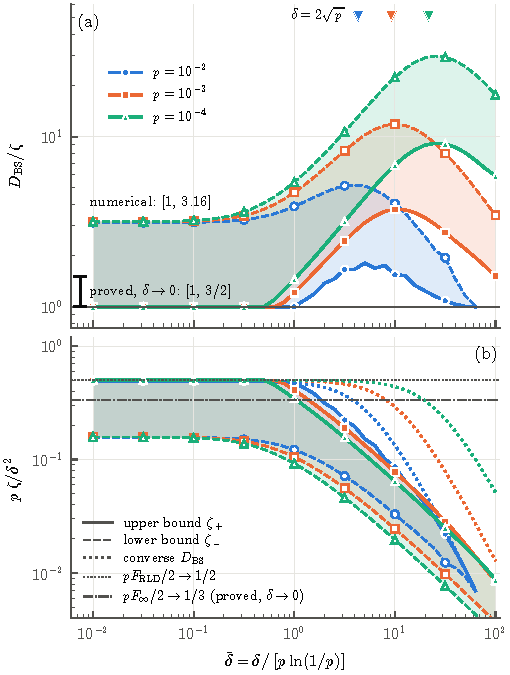
\includegraphics[width=0.8\linewidth]{fig3_crossover}
\caption{Crossover from genuine to spurious fragility for the adaptive Stein exponent $\zeta(\cN_{p,\delta}\|\cN_p)$ of a depolarized qubit gate, for $p=10^{-2},10^{-3},10^{-4}$, against $\bar\delta=\delta/[p\ln(1/p)]$. Here $\zeta_-\le\zeta\le\zeta_+$ are lower bounds from explicit finite-length strategies and certified upper bounds. (a) Ratio of the Belavkin--Staszewski converse to $\zeta$: solid lines divide by $\zeta_+$ and are certified lower bounds on the ratio; dashed lines divide by $\zeta_-$ and are upper bounds. For $\bar\delta\lesssim1$ the numerical bracket is $[1,3.16]$; the bar marks the narrower bracket $[1,\IR/\Iinf]\subset[1,3/2]$ that Eq.~\eqref{gate:eq:ratio} proves in the limit $\delta\to0$. Arrows mark $\delta=2\sqrt p$, near which the certified overshoot peaks. (b) $\zeta_\pm$ and $\DBS$ in units of $\delta^2/p$, with the local limits $p\Iinf/2\to1/3$ (a proved lower bound on $p\zeta/\delta^2$ as $\delta\to0$) and $p\IR/2\to1/2$. Below $\delta\approx p\ln(1/p)$ the converse follows $\zeta$; above it, the converse exceeds $\zeta$ by a factor that grows as $p$ decreases.}
\label{gate:fig:crossover}
\end{figure}

\emph{Chernoff exponent.} Symmetric discrimination behaves in the same way. Here $\hat C=-\ln\Fg\simeq\IR\delta^2/8$, and the argument behind Eq.~\eqref{gate:eq:ratio}, with the quantum Chernoff bound in place of the relative entropy, gives $\Iinf/8\le\liminf_{\delta\to0}\xi/\delta^2\le\limsup_{\delta\to0}\xi/\delta^2\le\IR/8$, so $1\le\hat C/\xi\le\IR/\Iinf<3/2$ as $\delta\to0$ (Proposition~\ref{gate:prop:m1local} in Chapter~\ref{gate:proofschapter}). Single-use strategies reach only $\xi\approx\delta^2/4$, without the factor $1/p$, so the $1/p$ curvature again comes from adaptive accumulation with error detection. At finite $\delta$ we bound $\xi$ by refereed one-copy converses evaluated at the midpoint $\delta/2$. The certified overshoot $\hat C/\xi$ then reaches $1.13$, $2.48$ and $6.00$ for $p=10^{-2}$, $10^{-3}$ and $10^{-4}$, near $\delta\approx2.9\sqrt p$, and as $p\to0$ it is at least $0.27/(\sqrt p\ln(1/p))$.

\begin{table}[!tbp]
\centering
\small
\caption{Genuine and spurious fragility of the converses, by sense of sensitivity and task. ``Genuine'' means that the operational exponent has the same sensitivity as the converse (up to the stated factor); ``spurious'' means that only the converse has it. The first row concerns amplitude damping, the second the worst case of Theorem~\ref{gate:thm:floor}, and the last two the depolarized qubit gate $(\cN_{p,\delta},\cN_p)$; under biased noise the local ratio stays below $2$ for single-qubit errors, and for correlated two-qubit errors the local bracket widens to $2/p$ (Sec.~\ref{gate:sec:physical}).}
\label{gate:tab:verdict}
\begin{tabular}{p{0.21\textwidth}p{0.335\textwidth}p{0.335\textwidth}}
\toprule
regime & Stein: $\zeta$ vs.\ $\DBS$ & Chernoff: $\xi$ vs.\ $\hat C$ and $-2\ln\Fg$\\
\midrule
Choi supports (Sec.~\ref{gate:sec:regimes}) & genuine: $\zeta(\cA_\gamma\|\cA_{\gamma'})=\infty$ & spurious: converses $=\infty$ while $\xi\to0$\\
first order, per unit of $\dn{\Psi'-\Psi}$ & genuine: both at most $1/(2\ltil)$, equal at the worst case & genuine: both at most $1/(2\ltil)$, equal at the worst case\\
second order, $\delta\lesssim p\ln(1/p)$ & genuine: $1\le\DBS/\zeta\le\IR/\Iinf<3/2$ as $\delta\to0$ & genuine: $1\le\hat C/\xi\le\IR/\Iinf<3/2$ as $\delta\to0$\\
second order, $p\ln(1/p)\lesssim\delta\lesssim\sqrt p$ & spurious: $\DBS/\zeta$ up to $1.81$, $3.74$, $9.15$ for $p=10^{-2},10^{-3},10^{-4}$; $\approx0.8/(\sqrt p\ln\frac1p)$ & spurious: $\hat C/\xi$ up to $1.13$, $2.48$, $6.00$ for $p=10^{-2},10^{-3},10^{-4}$; $\approx0.5/(\sqrt p\ln\frac1p)$\\
\bottomrule
\end{tabular}
\end{table}

Table~\ref{gate:tab:verdict} collects the verdicts. The crossover has a simple origin. The exponent grows at least as $\delta^2/(3p)$, and at most as $\delta^2/(2p)$, only until it reaches its own continuity bound, which is of order $\delta\ln(1/p)$; this happens at $\delta\sim p\ln(1/p)$. Beyond that point $\zeta$ grows at most linearly in $\delta$, whereas $\DBS$ continues to grow as $\delta^2/(2p)$ until $\Fg$ approaches saturation at the window $\delta\sim\sqrt p$ of Eq.~\eqref{gate:eq:delta}. The three regimes of Sec.~\ref{gate:sec:regimes} thus reappear at a noisy gate on three scales: genuine fragility for $\delta\lesssim p\ln(1/p)$, a spurious overshoot that grows up to its peak near $\delta\approx2\sqrt p$, and saturation beyond, where the overshoot recedes. For estimation, which probes the local regime, the $1/p$ curvature of the RLD-type bounds is physical. For discrimination of gates that differ by more than $p\ln(1/p)$, it is mostly an artifact of single-letter bounds. A better target is then $\zeta$ itself, which is computable~\cite{SchmittSutter2026,WangYang2026} although no convergence rate is known, or its continuity bound.

\section{Certification from finite data}\label{gate:sec:cert}

A converse computed from a tomographic estimate is a statement about the estimate. To make it a statement about the device, one needs a confidence region and a bound valid on all of it. Equation~\eqref{gate:eq:r} provides this.

\begin{theorem}[Certified converse]\label{gate:thm:cert}
Suppose that, with probability at least $1-\alpha$, the true channels lie within diamond distance $\epsilon$ of channel estimates $\hat\Phi,\hat\Psi$ (completely positive and trace preserving) whose Choi floors are at least $\hat\lambda$, and let $r=d_X\epsilon/(2\hat\lambda)<1$. Then, with the same probability, the true floors are at least $(1-r)\hat\lambda$ and
\begin{equation}\label{gate:eq:cert}
\xi(\Phi,\Psi)\le\hat C(\Phi,\Psi)\le\hat C(\hat\Phi,\hat\Psi)+\ln\frac{1}{1-r}.
\end{equation}
\end{theorem}

An analogous bound for $\zeta$ adds the continuity bound of Sec.~\ref{gate:sec:laws} to $\DBS(\hat\Phi\|\hat\Psi)$ (Chapter~\ref{gate:proofschapter}, Section~\ref{gate:sec:cert-proofs}). Both bounds are one-sided in the direction that keeps the converse valid, which is the direction that matters for certification. Plug-in values carry no such guarantee. In our simulations the plug-in $\Fg$ exceeded the true value, which makes the converse claim a stronger limit than is true, in up to $32\%$ of runs for linear inversion, depending on $p$ and the sample size, and in up to $96\%$ of runs for a hedged maximum-likelihood estimate~\cite{BlumeKohout2010} at small sample sizes (Section~\ref{gate:sec:cert-proofs}).

By the sharpness in Eq.~\eqref{gate:eq:sharp}, a diamond ball of radius $\epsilon$ contains pairs whose values of $\ln\Fg$ differ by $\epsilon/(4\ltil)$, so an additive accuracy $\eta$ requires $\epsilon\lesssim4\eta\ltil$. Diamond-norm tomography~\cite{MeleBittel2025} reaches this with $O\big((d_Xd_Yk+d_X\ln\frac1{\alpha})/(\eta\ltil)^2\big)$ uses for channels of Kraus rank $k$; this learner is coherent, since it processes the channel outputs jointly. For learners that measure each channel output separately, possibly choosing later inputs from earlier outcomes, no strategy reaches diamond accuracy $\epsilon$ on the gate family of Eq.~\eqref{gate:eq:gate} with fewer than order $1/\epsilon^2$ uses (Proposition~\ref{gate:prop:N12}(b) in Chapter~\ref{gate:proofschapter}; see also Ref.~\cite{OufkirGirardi2026}), hence order $1/(\eta\ltil)^2$. For such incoherent learners, certification through a diamond ball therefore costs order $1/(\eta\ltil)^2$ uses. Whether coherent learners can do better is open. The two-point argument behind the incoherent bound does not extend to them: with error-corrected coherent probing the Fisher information per use for the rotation angle is $\Iinf\approx2/(3p)$, and the same argument then gives only order $p/\epsilon^2\approx1/(\eta^2p)$ uses, no more than the intrinsic cost below.

This cost is not intrinsic to the task. For Pauli channels the relevant information sits in the error rate $q$ of a floor sector, and a relative change $\eta$ of $q$ carries information of order $\eta^2q$ per use. For local depolarizing noise, any strategy, adaptive or coherent, needs at least $0.0246/(\eta^2\ltil)$ uses to estimate $\Fg(\mathrm{Ad}_{PU},\Psi)$, the fidelity of the noisy gate with a correlated error of full weight, to relative accuracy better than $\eta\le0.1$. Bell-basis estimation of the Pauli error rates in a known frame~\cite{FlammiaWallman2020,HarperFlammiaWallman2020} achieves $O(\ln(1/\alpha)/(\eta^2\ltil))$. The separation is therefore between variance-blind confidence regions, whose radius is set by the largest outcome variances, and variance-adaptive ones, whose width in the floor directions shrinks with the floor; it is not specific to the diamond norm. We conjecture that $\tilde O(\mathrm{poly}(d)/(\eta^2\ltil))$ uses suffice for all channel pairs.

\begin{figure}[!tbp]
\centering
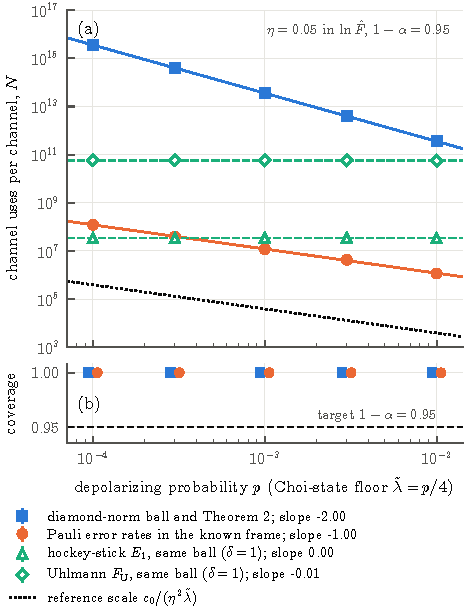
\includegraphics[width=0.8\linewidth]{fig4_cert}
\caption{Cost of certifying converses from simulated single-qubit Pauli tomography. (a) Channel uses per channel for a certified lower bound on $\Fg(\cN_{p,\delta},\cN_p)$ at $\delta=2\sqrt p$, i.e., an upper bound on the converse $-\ln\Fg$, to accuracy $\eta=0.05$ at confidence $1-\alpha=0.95$ (median run; error bars are bootstrap intervals, lines are fits). A variance-blind diamond-norm ball combined with Theorem~\ref{gate:thm:cert} costs order $p^{-2}$ by construction; variance-adaptive estimation of the Pauli error rates in the known frame costs order $p^{-1}$. Through the same ball, the hockey-stick divergence and the Uhlmann fidelity at $\delta=1$ cost the same at every $p$. The dotted line is the reference scale $c_0/(\eta^2\ltil)$, proved as a lower bound for the related estimand $\Fg(\mathrm{Ad}_{PU},\Psi)$, not for the pair simulated here. (b) Empirical coverage of the certified bounds in 1000 runs per point; the target is $0.95$.}
\label{gate:fig:cert}
\end{figure}

Simulations of single-qubit Pauli tomography illustrate both scalings (Fig.~\ref{gate:fig:cert}). For the pair with $\delta=2\sqrt p$, where $\Fg\approx0.71$, we certified a lower bound on $\Fg$, hence an upper bound on the converse, to accuracy $\eta=0.05$ in $\ln\Fg$ at $95\%$ confidence. In the first procedure, Theorem~\ref{gate:thm:cert} is applied to a diamond-norm ball around the linear-inversion estimate, whose Hoeffding radius does not adapt to the small outcome probabilities in the floor directions. Its cost, $3.6\times10^{13}$ uses per channel at $p=10^{-3}$, follows from that radius by construction and is proportional to $p^{-2}$. In the second procedure, the Pauli error rates are estimated directly in the known frame with exact binomial intervals, and $\Fg$ is minimized exactly over the resulting confidence polytope; the cost grows as $p^{-1.00\pm0.04}$ and is $1.2\times10^{7}$ uses at $p=10^{-3}$. The certified bounds held in all 1000 repetitions at every $p$. Through the same diamond ball, the hockey-stick divergence and the Uhlmann fidelity are certified with a number of uses independent of $p$. Bounds of the opposite type, which limit distinguishability from below, show the same separation: variance-blind isotropic regions cost order $p^{-2}$, whereas a box of exact binomial intervals on the setting probabilities, which is variance-adaptive and needs no model assumption, already costs order $p^{-1}$ (Chapter~\ref{gate:proofschapter}, Section~\ref{gate:sec:cert-proofs}). The second procedure assumes Pauli noise in the known frame; whether model-free tomography attains the $1/\ltil$ law on the converse side is open. For a two-qubit CNOT gate under local noise, plug-in (not certified) estimates of $\Fg$ needed a number of shots growing approximately as $p^{-4}\propto1/\lambda^2$, with $\lambda=p^2/4$, in line with the multi-qubit floor (three points on a one-decade grid).

\section{Discussion}\label{gate:sec:discussion}

The sensitivity of geometric channel divergences near noisy gates has two senses. At first order, a diamond-norm error in the model moves the converses by up to order $1/\ltil$ per unit of distance, with the sharp constant of Theorem~\ref{gate:thm:floor}. At the worst case the adaptive exponents move at the same rate (Proposition~\ref{gate:prop:worst}), so in this sense the sensitivity belongs to the task, and a first-order gap between converse and exponent requires a converse that is already loose.
At second order, the curvature of the converses in a coherent miscalibration grows as $1/p$. In this sense the sensitivity has two sources. One is physical: adaptive strategies can exploit the noise floor, and the Stein and Chernoff exponents and the error-corrected Fisher information inherit a $1/p$ scale for small miscalibrations. The other is an artifact of single-letter bounds, which keep the $1/p$ curvature well beyond the point where the exponent has crossed over to its $\ln(1/p)$ continuity bound, and which can be infinite where the exponent vanishes. For an experimentalist the practical consequences are concrete. A converse computed from a pure-$T_1$ or noiseless model can be infinite for reasons that have nothing to do with the device; the residual thermal population or depolarizing floor sets its value and must be part of the model. Error budgets for geometric converses must be set relative to the Choi floor, which for $n$ qubits under local noise is $(p/4)^n$, and, for a given miscalibration, relative to the rate of the corresponding Pauli error, which under biased noise can be far smaller than the dominant error rate. And confidence regions should be variance-adaptive rather than isotropic in the diamond norm, which for Pauli channels saves a factor of order $1/\ltil$ in data.

Several questions remain open. We do not know whether Conjecture~\ref{gate:conj:32} holds, where in its bracket the local Chernoff coefficient lies, whether unitary channels give the worst-case slope of $\Fg$, whether the exponent inherits the narrow window of the converses for correlated multi-qubit errors, whether coherent learners can certify through a diamond ball with fewer than order $1/(\eta\ltil)^2$ uses, or whether the intrinsic certification cost is of order $1/(\eta^2\ltil)$ for all channels. For amplitude damping, the conjectured bound $\xi\le-2\ln f$ would pin $\xi$ within a factor two. A single-letter converse that stays finite at spurious pairs, such as $\min\{\hat C,C_{\rm bar},-2\ln\mu_*\}$, and the extension of these laws to bosonic loss channels with energy constraints, are natural next steps.

\section{Plan of the book}\label{gate:sec:plan}
The rest of the book develops the theory behind this chapter. Chapter~\ref{ov:chapter} is an overview: it explains the three classical ``shadows'' of a pair of states or channels that organize the theory, summarizes the main results of each chapter, shows how the chapters depend on each other and suggests reading orders. Chapter~\ref{nt:chapter} fixes the notation and records where the conventions of the chapters differ. Chapter~\ref{cont:chapter} introduces the Arveson--Radon--Nikodym derivative of a pair of channels and proves the continuity dichotomy and the Choi-floor estimates used in Sections~\ref{gate:sec:regimes} and~\ref{gate:sec:laws}. Chapter~\ref{shA:chapter} treats testing regions and hockey-stick divergences and proves the continuity properties of the adaptive Stein exponent used in Sections~\ref{gate:sec:regimes} and~\ref{gate:sec:laws}; Chapter~\ref{shB:chapter} studies the super-multiplicativity of the hockey-stick R\'enyi quasi-entropies under tensor products. Chapter~\ref{chn:chapter} describes adaptive discrimination as a controlled random walk and proves the geometric Chernoff converse of Eq.~\eqref{gate:eq:converses2} and the fragility of single-letter Chernoff converses discussed in Section~\ref{gate:sec:regimes}. Chapter~\ref{gate:proofschapter} contains the proofs of the results stated in this chapter, together with closed forms for Pauli channels, the analysis of amplitude damping, the certification bounds and the numerical methods. Chapter~\ref{op:chapter} collects the open problems of all chapters, including those listed above.

\endgroup
